\documentclass{article}
\usepackage{amsmath}
\usepackage{amssymb}
\usepackage{tikz}
\usepackage{geometry}
\geometry{margin=1in}

\title{\vspace{-1cm}Infinitesimal Calculus\vspace{-0.5cm}}
\date{}


\begin{document}
\maketitle

\vspace{-1cm}

\textbf{Definition}: An \textbf{infinitesimal} is a quantity that is closer to zero than any
standard real number but is not zero itself.

\textbf{Theorem}: If $\alpha$ is an infinitesimal, then $\alpha \notin \mathbb{R}$.

\textbf{Proof}: Let $\alpha$ be an infinitesimal. Clearly there are smaller positive real numbers than $\alpha$.

\begin{center}
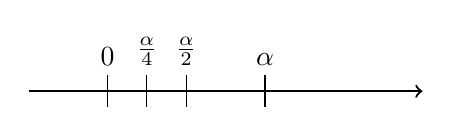
\begin{tikzpicture}[scale=2]
    % Draw the number line
    \draw[->,thick] (-0.5,0) -- (2,0);
    
    % Add tick marks and labels
    \draw (0,-0.1) -- (0,0.1) node[above] {$0$};
    \draw (1,-0.1) -- (1,0.1) node[above] {$\alpha$};
    
    % Add infinitesimals (exaggerated for visibility)
    \draw (0.5,-0.1) -- (0.5,0.1) node[above] {$\frac{\alpha}{2}$};
    \draw (0.25,-0.1) -- (0.25,0.1) node[above] {$\frac{\alpha}{4}$};
    


\end{tikzpicture}
\end{center}

Therefore, infinitesimals do not exist.

\section*{Geometric Approach to the Derivative of \(x^2\)}

When we increase the side length of a square from $x$ to $x + dx$, the change in area can be seen geometrically:


\begin{center}

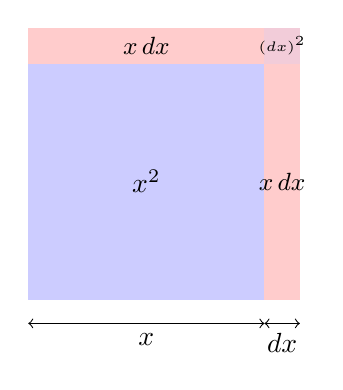
\begin{tikzpicture}[scale=1.5]
    % Original square
    \fill[blue!20] (0,0) rectangle (2,2);
    
    % Additional rectangles
    \fill[red!20] (2,0) rectangle (2.3,2);
    \fill[red!20] (0,2) rectangle (2,2.3);
    
    % Small square at corner
    \fill[purple!20] (2,2) rectangle (2.3,2.3);
    
    % Labels
    \node at (1,1) {$x^2$};
    \node at (2.15,1) {\small$x\,dx$};
    \node at (1,2.15) {\small$x\,dx$};
    \node at (2.15,2.15) {\tiny$(dx)^2$};
    
    % Dimensions
    \draw[<->] (0,-0.2) -- (2,-0.2) node[midway,below] {$x$};
    \draw[<->] (2,-0.2) -- (2.3,-0.2) node[midway,below] {$dx$};
\end{tikzpicture}
\end{center}

The total change in area $dA$ is:
\[ dA = 2x\,dx + (dx)^2 \]

Remember that $A = x^2$

\[
\begin{aligned}
    dA &= 2x\,dx + (dx)^2 \\
    dx^2 &= 2x\,dx + (dx)^2 \\
    \frac{dx^2}{dx} &= \frac{2x\,dx + (dx)^2}{dx} \\
    \frac{d}{dx}(x^2) &= 2x + dx \quad \text{(dx is basically 0)} \\
    \frac{d}{dx}(x^2) &= 2x
\end{aligned}
\]


Where:
\begin{itemize}
    \item $2x\,dx$ represents the two red rectangles (each with area $x\,dx$)
    \item $(dx)^2$ represents the tiny purple square at the corner
\end{itemize}

Since $dx$ is infinitesimal, $(dx)^2$ is "even more infinitesimal" and can be ignored:
\[ \frac{dA}{dx} \approx 2x \]

\section*{Why This Works Geometrically}

\begin{center}
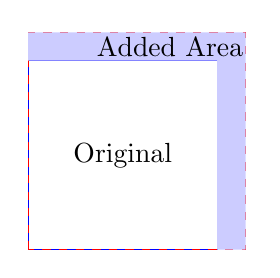
\begin{tikzpicture}[scale=1.2]
    % Before and after squares
    \draw[blue] (0,0) rectangle (2,2);
    \draw[red,dashed] (0,0) rectangle (2.3,2.3);
    
    % Shading for area difference
    \fill[blue!20] (2,0) -- (2.3,0) -- (2.3,2.3) -- (0,2.3) -- (0,2) -- (2,2) -- cycle;
    
    \node at (1,1) {Original};
    \node at (1.5,2.15) {Added Area};
\end{tikzpicture}
\end{center}

The derivative represents the rate of change of area with respect to side length:
\begin{itemize}
    \item As $dx \to 0$, the purple corner square becomes negligible
    \item Added area $\approx$ two rectangular strips of width $dx$ and length $x$
    \item Thus, instantaneous rate of change = $2x$
\end{itemize}

This geometric approach shows why the derivative of $x^2$ is $2x$ in a visual, intuitive way that matches our understanding of area.

\section*{Alternate Geometric Approach to the Derivative of \(\sqrt{x}\) via a Circular Sector}

Let 
\[
r=\sqrt{x} \quad\Longrightarrow\quad x=r^2.
\]
Now, consider a circular sector with radius \(r\) and a fixed central angle \(\theta = 2\) radians. (Note that using \(\theta=2\) makes the area of the sector equal to
\[
A=\frac{\theta}{2\pi}\cdot\pi r^2=\frac{2}{2\pi}\pi r^2=r^2=x.
\]
) Now, if we change the radius by an infinitesimal amount 
\[
dr=d\sqrt{x},
\]
the corresponding change in area is approximately the area of a thin annular (ring‐like) sector. This small area is given by the product of the "arc length" of the sector and \(dr\). Since the arc length of a sector is
\[
s=r\,\theta=2r,
\]
we have
\[
dA\approx s\,dr=2r\,dr.
\]
But because \(A=x\), also \(dA=dx\) and therefore
\[
dx\approx 2r\,d\sqrt{x}.
\]
Dividing both sides by \(dx\) (and taking the infinitesimal limit) gives
\[
\frac{d\sqrt{x}}{dx} \approx \frac{1}{2r}=\frac{1}{2\sqrt{x}},
\]
which is exactly the derivative of \(\sqrt{x}\).

\vspace{-0.5cm}

\begin{center}
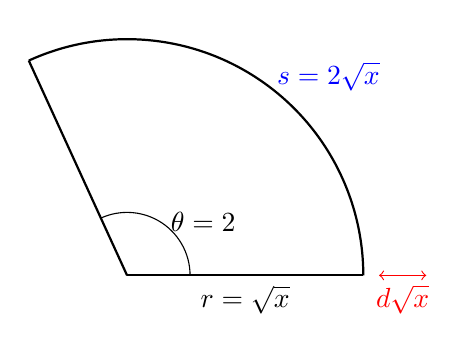
\begin{tikzpicture}[scale=1]
    % Define the center and a sample radius (r = 3 for illustration)
    \coordinate (O) at (0,0);
    \def\r{3}
    
    % Draw the two radii defining the circular sector.
    \draw[thick] (O) -- (\r,0) node[midway, below] {\(r=\sqrt{x}\)};
    \draw[thick] (O) -- ({\r*cos(114.59)},{\r*sin(114.59)});
    
    % Draw the arc of the sector from 0 to 114.59°.
    \draw[thick] (\r,0) arc (0:114.59:\r);
    
    % Annotate the central angle.
    \draw (0.8,0) arc (0:114.59:0.8) node[midway, right] {\(\theta=2\)};
    
    % Label the arc length: s = r*θ = 2r.
    \path (O) ++({1.1*\r*cos(57.3)},{\r*sin(57.3)}) node (midarc) {};
    \node[blue, right] at (midarc) {\(s=2\sqrt{x}\)};
    
    % Draw a red arrow along the radius to illustrate the differential change dr.
    \draw[<->, red] (\r+0.2,0) -- node[below] {\(d\sqrt{x}\)} (\r+0.8,0);
\end{tikzpicture}
\end{center}

\end{document}